\documentclass[./main.tex]{subfiles}

\begin{document}
\section{Analisi esplorativa}
Per condurre una prima analisi esplorativa si sono considerati i grafici dell'accelerazione rispetto al tempo (ms) per le diverse attività registrate; da ogni misurazione sono stati tolti i primi e gli ultimi sette secondi ottenendo le seguenti rappresentazioni:
\begin{figure}[H]
	\centering
	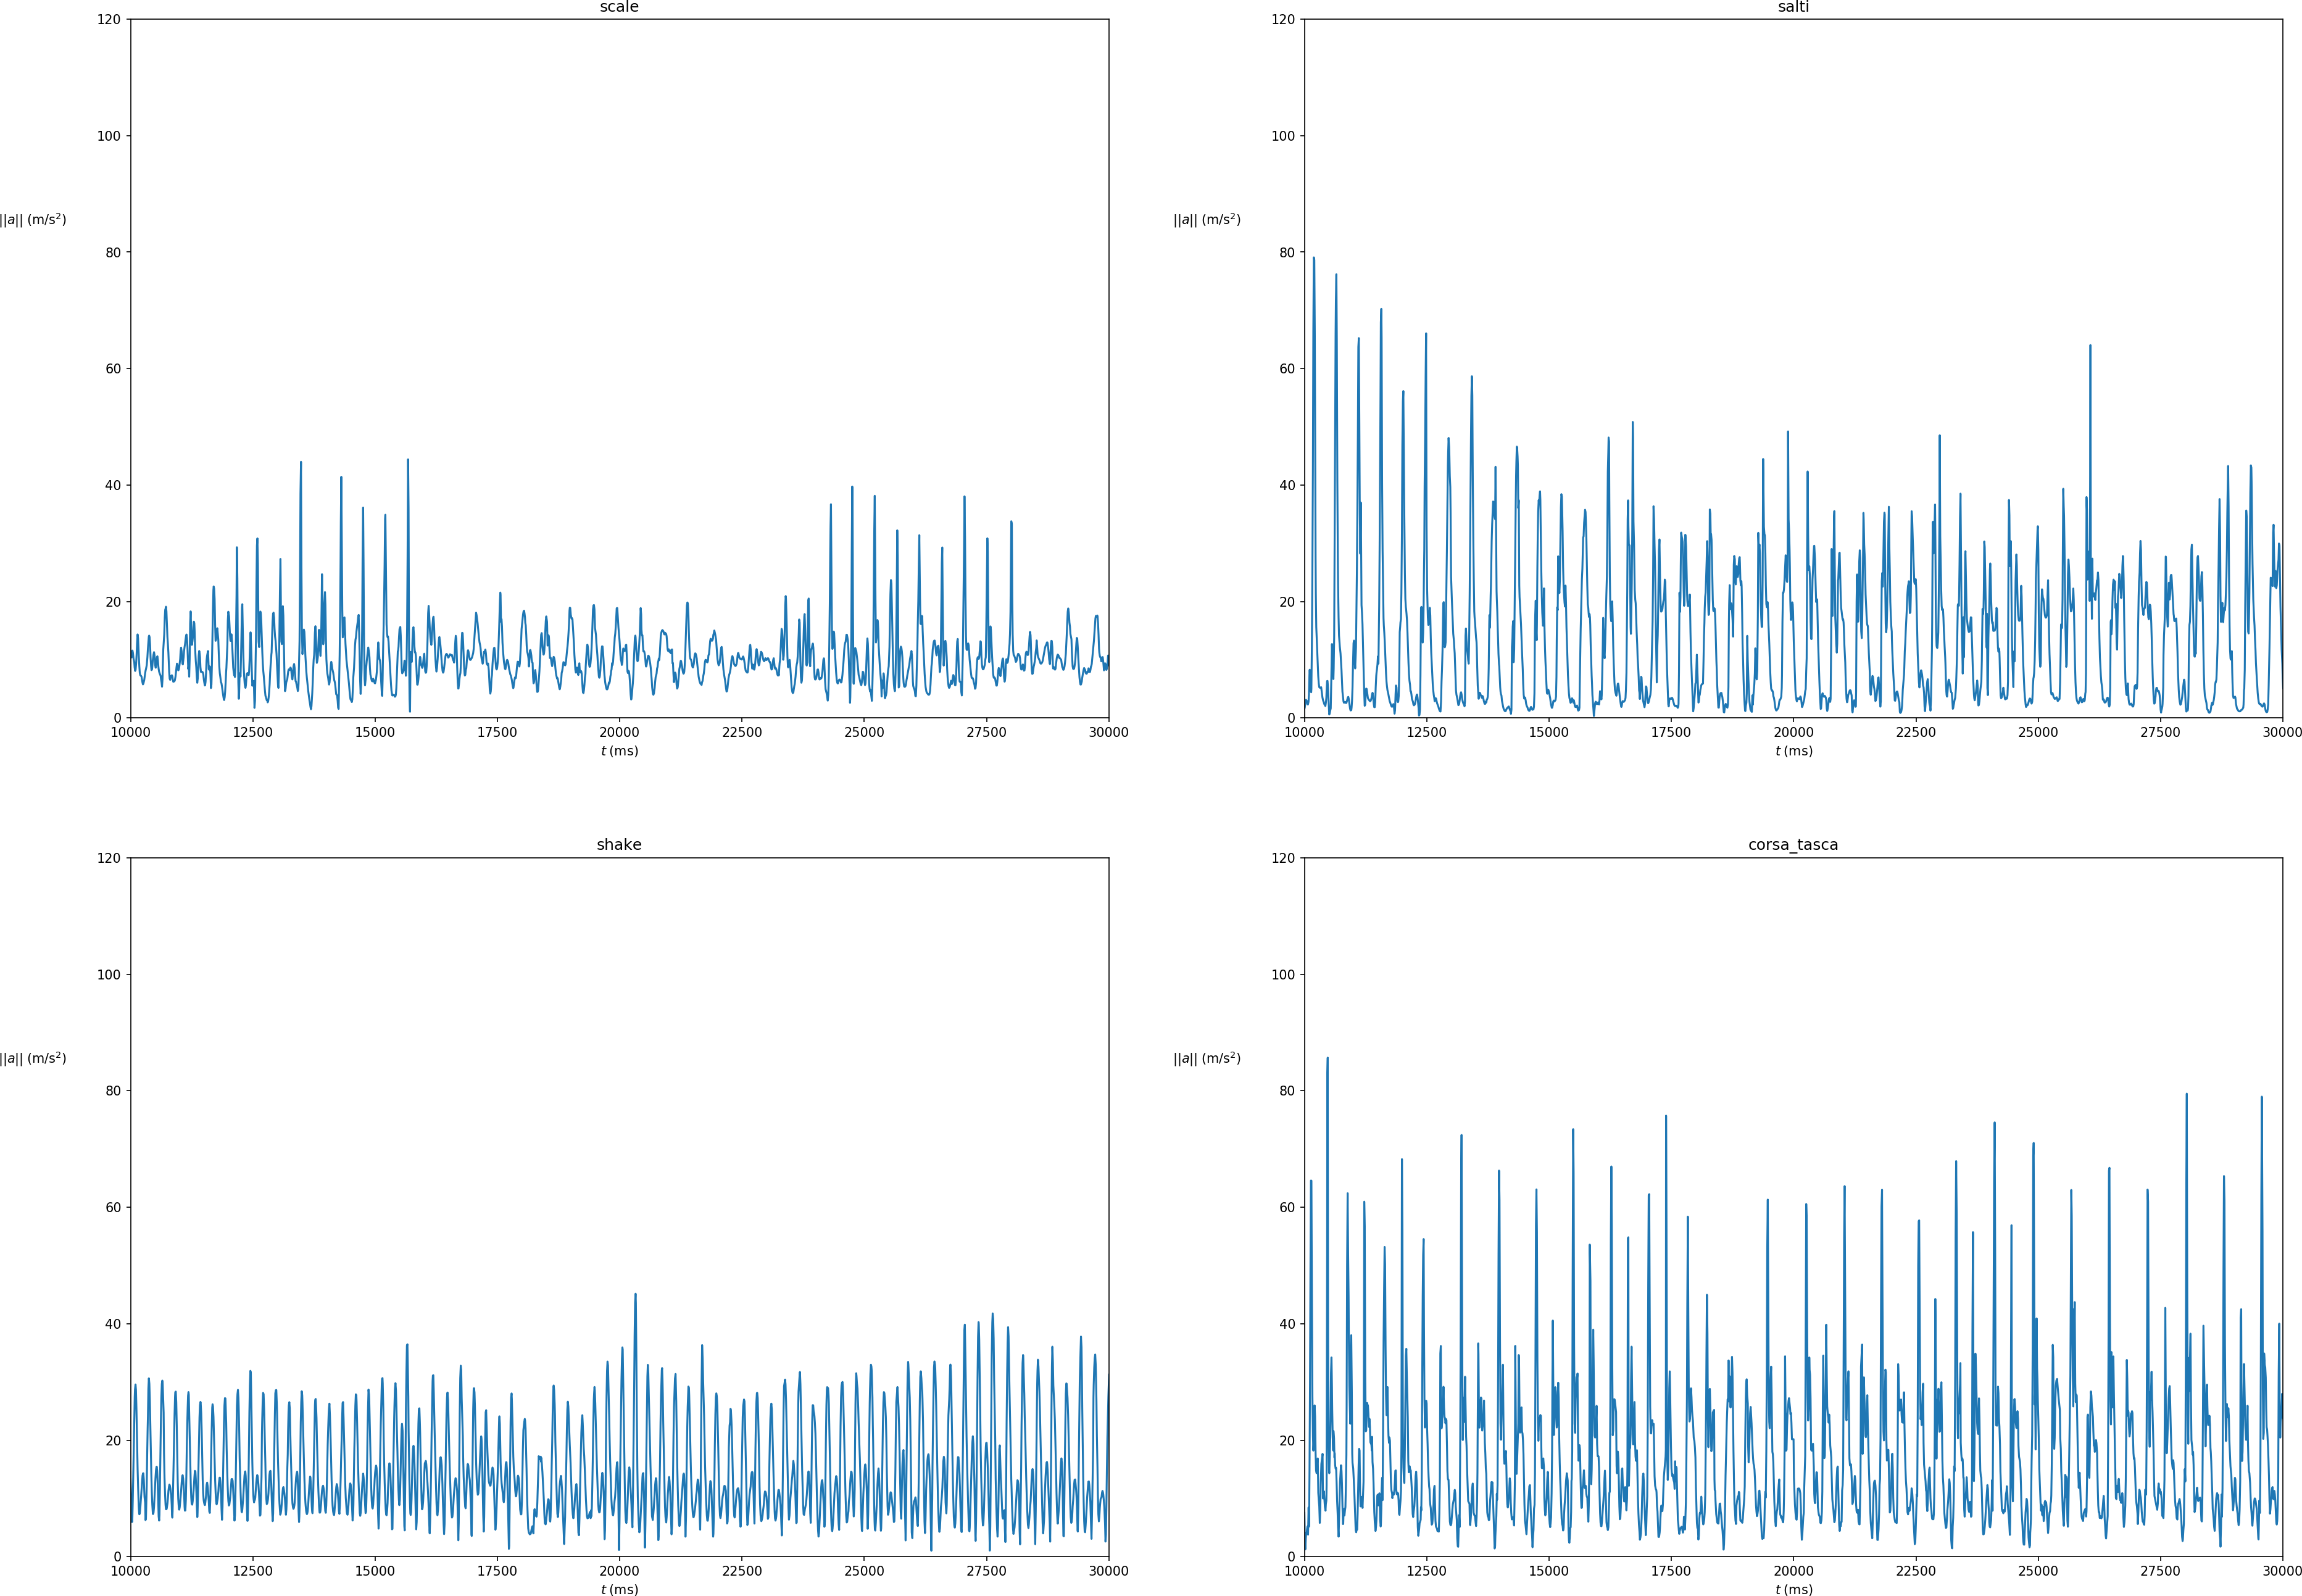
\includegraphics[width=.8\textwidth, keepaspectratio]{../../figure/espl.png}
	\caption{{}}
	\label{espl}
\end{figure}
In generale, per le varie attività registrate si osserva che l'intensità dell'accelerazione e la frequenza dei picchi sono entrambe piuttosto basse per "camminata", "camminata tasca", "corsa" e "quotidiano". La differenza inizia ad emergere nello studio di "salti", "corsa tasca" e "shake".\\
Emerge chiaramente come il segnale sia molto differente per queste tre diverse attività. In particolare si nota
una differenza nell'intensità (più bassa per lo shake e maggiore negli altri due casi) e nella frequenza (la quale cresce passando da "cosa tasca" a "salti" fino a "shake"). Anche i picchi che vengono raggiunti sono diversi nei vari casi: nel primo si hanno picchi fino a $90\si{\metre\per\square\second}$ ma poco frequenti; nel secondo si notano picchi di intensità lievemente inferiore ma molto più ravvicinati. Infine lo shake evidenzia un segnale molto denso con  picchi piuttosto bassi rispetto ai precedenti.\\
Ciascun segnale è stato suddiviso in intervalli di ampiezza \SI{1.5}{s}, sui quali sono state calcolate le seguenti variabili riassuntive:
\begin{table}[H]
	\begin{tabular}{ll}
%		\texttt{meanA}& Media dell'accelerazione.\\
		\texttt{medianA}& Mediana dell'accelerazione.\\
		\texttt{varA}& Varianza dell'accelerazione.\\
		\texttt{maxA}& Massimo dell'accelerazione.\\
		\texttt{intTrapz}& Integrale del segnale nell'intervallo, calcolato con l'approssimazione per trapezi \textbf{CIT}.\\
		\texttt{MVDeriv}& Media della variazione assoluta della derivata \textbf{CIT}.
	\end{tabular}
\end{table}
Successivamente sono stati sbiancati i dati e sono state applicate le seguenti tecniche d'analisi:
\begin{itemize}
	\item PCA sui dati sbiancati.
	\item ICA sui dati sbiancati.
	\item t-SNE sui dati sbiancati.
\end{itemize}
Le prime due componenti principali non riescono a isolare adeguatamente i vari segnali; l'analisi delle componenti indipendenti non migliore il risultato dal momento che quest'ultima rappresenta una rotazione della prima. Un output migliore lo si ottiene mediante il t-SNE (figura \ref{t-sne}). 
\begin{figure}[H]
	\centering
	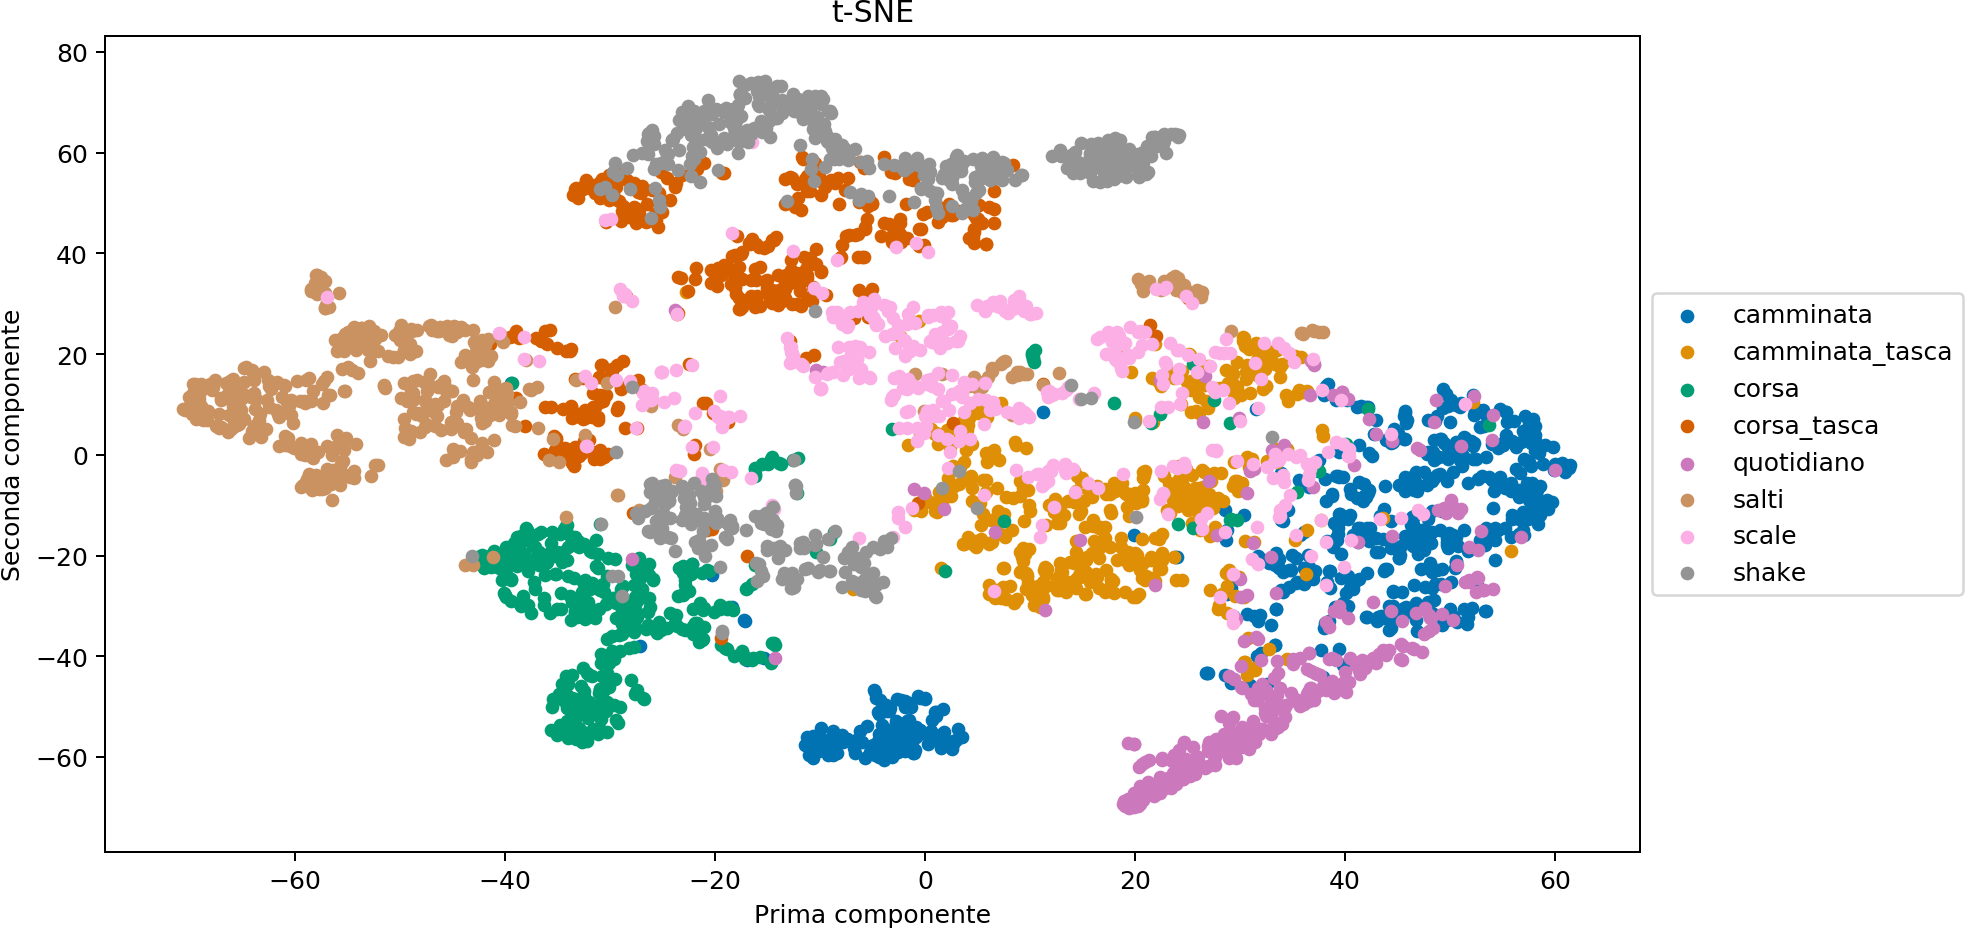
\includegraphics[width=.8\textwidth, keepaspectratio]{../../figure/t-SNE.png}
	\caption{{ t-SNE per i dati sbiancati}}
	\label{t-sne}
\end{figure}
Si osserva in particolare come l'attività di interesse, ovvero lo shake, venga principalmente confusa con "corsa" e "corsa tasca". 
\\
Tale problema rappresenta il punto di partenza per un'analisi volta a classificare correttamente i vari segnali nelle diverse categorie.

\textcolor{red}{EVENTUALE COMMENTO SULLE DISTRIBUZIONI DELLE ESPLICATIVE SCELTE}
\end{document}